\documentclass{beamer}

% Theme and color settings (professional and "space" oriented)
\usetheme{Madrid}
\usecolortheme{whale}

% Necessary packages
\usepackage[utf8]{inputenc}
\usepackage[english]{babel}
\usepackage{graphicx}
\usepackage{booktabs}
\usepackage{listings}


% Presentation Metadata
\title[Lunar Rover XRF Classification]{Lunar Surface Analysis via XRF}
\author{Casadio Sara, Ferraiolo Enrico, Gianlorenzo Urbano}
\institute{Alma Mater Studiorum - University of Bologna}
\date{May 11, 2026}

\begin{document}

% --- Title Slide ---
\begin{frame}
    \titlepage
\end{frame}

% --- Table of Contents ---
\begin{frame}{Outline}
    \tableofcontents
\end{frame}

% --- Section 1: Introduction ---
\section{Introduction}
\begin{frame}{Introduction}
    \begin{itemize}
        \item \textbf{Goal:} Identification and quantification of chemical elements on the lunar surface to support future exploration.
        \item \textbf{The Challenge:} Remote sensing via X-ray Fluorescence (XRF) produces complex, noisy, and high-dimensional spectral data.
        \item \textbf{Methodology:} Using Machine Learning to automate and refine the interpretation of these spectra.
        \item \textbf{Data Strategy:} Development of a custom dataset and utilization of \texttt{multiel-spectra} for high-fidelity synthetic data generation.
    \end{itemize}
\end{frame}

\begin{frame}{XRF Spectroscopy Fundamentals}
    \begin{columns}
        \column{0.5\textwidth}
        \begin{itemize}
            \item High-energy X-rays/Gamma rays irradiate the sample.
            \item Secondary X-rays (fluorescence) are emitted, unique to each element.
            \item The detector captures a spectrum where energy peaks correspond to specific atoms.
        \end{itemize}
        \column{0.5\textwidth}

        \begin{figure}
            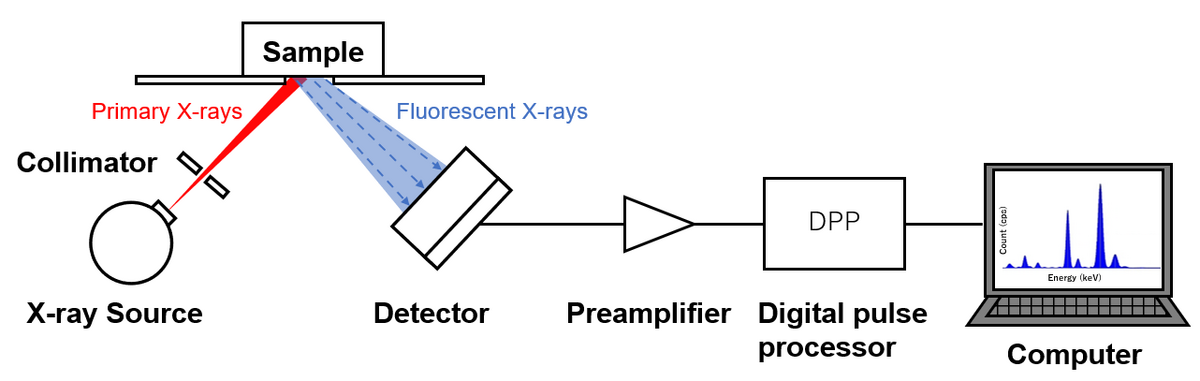
\includegraphics[width=\linewidth]{Media/xrf_diagram.png}
        \end{figure}

    \end{columns}
\end{frame}

% --- Section 2: Objectives ---
\section{Classification Goals}
\begin{frame}{Phase 1: Element Classification}
    Classification aims to answer: \textbf{"Which elements are present in this sample?"}
    \vspace{0.3cm}
    \begin{block}{Research Focus}
        \begin{enumerate}
            \item \textbf{Multi-Element Identification:} Detecting one or more elements simultaneously (Multi-label classification).
            \item \textbf{Model Robustness:} Evaluating accuracy across different anode target materials.
            \item \textbf{Detection Thresholds:} Determining the minimum "thinness" (concentration) for reliable element detection.
        \end{enumerate}
    \end{block}
\end{frame}

% --- Section 3: Methodology ---
\section{Methodology \& Synthetic Data}
\begin{frame}{Data Generation: multiel-spectra}
    To simulate lunar conditions, we vary key hardware and environmental parameters:
    \begin{itemize}
        \item \textbf{Target Materials:} Mo (Molybdenum), Rh (Rhodium), W (Tungsten).
        \item \textbf{Filters:} Simulating different rover shielding configurations.
        \item \textbf{Noise Profile:} Applying Poisson noise and background radiation to mimic the space environment.
    \end{itemize}
    \begin{exampleblock}{Sample Configuration}
        \texttt{s\_counts\_range: (10000, 30000)} \\
        \texttt{min\_elements: 1, max\_elements: 5}
    \end{exampleblock}
\end{frame}

\begin{frame}{Model Architectures under Evaluation}
    Processing spectra as 600-bin vectors using various approaches:
    \begin{itemize}
        \item \textbf{Standard ML:} Random Forest, XGBoost (Baseline).
        \item \textbf{Deep Learning:} 
            \begin{itemize}
                \item MLP (Multi-Layer Perceptron).
                \item 1D CNN (to capture local peak correlations).
                \item Transformer-based models for spectral signatures.
            \end{itemize}
    \end{itemize}
\end{frame}

% --- Section 4: Parametric Analysis ---
\section{Parametric Analysis}
\begin{frame}{Anode Impact and Sensitivity Analysis}
    \begin{itemize}
        \item \textbf{Anode Variation:} How does the excitation spectrum change? Different elements require specific anodes for optimal excitation.
        \item \textbf{Minimum Concentration:} Analyzing the sensitivity curve to define the limit of detection (LOD).
        \item \textbf{Visualization:}
    \end{itemize}
    \centering \textit{[Insert Plot: Accuracy vs. Element Concentration]}
\end{frame}

% --- Section 5: Conclusions ---
\section{Conclusions \& Next Steps}
\begin{frame}{Preliminary Conclusions}
    \begin{itemize}
        \item Classification acts as the "gatekeeper" for subsequent phases (Regression and Denoising).
        \item Expected Outcome: A model capable of identifying lunar chemical signatures despite high noise.
        \item Integration: Future synergy with the Denoising phase to improve precision on low-concentration samples.
    \end{itemize}
\end{frame}

\begin{frame}
    \centering
    \Huge Questions?
    \vspace{1cm}
    \normalsize
\end{frame}

\end{document}